\documentclass[12pt]{article} 
\usepackage{amsmath} 
\usepackage{amsfonts}
\usepackage{amssymb} 
\usepackage[utf8]{inputenc} 
\usepackage[T1,T2A]{fontenc}
\usepackage[english, russian]{babel} 
\usepackage{graphicx}
\usepackage{float}
\usepackage[left=2cm,right=2cm,top=2cm,bottom=2cm]{geometry}
\usepackage{wrapfig}
\usepackage{pgfplots} 
\usepackage{setspace} 
\usepackage{indentfirst}
\usepackage{subfigure} 
\usepackage{hyperref}

\hypersetup{
    colorlinks=true,
    linkcolor=red,
    urlcolor=magenta,
}

\graphicspath{{pictures}}

\title{ 
    Лабораторная работа 2.1.6 \\
    <<Эффект Джоуля-Томсона>>
}

\author{Балдин Виктор, Б01-303}

\begin{document}
    \maketitle
    \paragraph{Цель работы}
    \begin{enumerate}
        \item Определение изменения температуры углекислого газа при протекании
        через малопроницаемую перегородку при разных начальных значениях.
        \item Вычисление по результатам опытов коэффициентов Ван-дер-Ваальса 
        $a$ и $b$.
    \end{enumerate}
    \paragraph{Оборудование} Трубка с пористой перегородкой; труба Дьюара;
    термостат, термометры; дифференицальная термопара; микровольтметр; 
    балластный баллон; манометр.

    \section{Теоретическая часть}
    Рассмотрим стационарный поток газа между произвольными сечениями трубки
    и пористой перегородкой. Для 1 моля можно записать первое начало термодинамики:
    \begin{equation}
        A_1 - A_2 = \left(U_2 + \frac{\mu v_2^2}{2}\right) - \left(U_1 + \frac{\mu v_1^2}{2}\right),
        \label{term1}
    \end{equation}
    где $A_1 = P_1V_1$ -- работа над газом, необходимая для внесения его в 
    первое сечение трубки, $A_2 = P_2V_2$ -- работа газа по прохождению второго
    сечения. Используя уравнение \ref{term1}, получим: 
    \begin{equation}
        H_1 - H_2 = (U_1 + P_1V_1) - (U_2 + P_2V_2) = \frac{1}{2}\mu (v_2^2 - v_1^2)
    \end{equation}
    Или:
    \begin{equation}
        C_P(T_1 - T_2) = \frac{1}{2}\mu (v_2^2 - v_1^2),
    \end{equation}
    откуда:
    \begin{equation}
        \Delta T = \frac{\mu}{2C_P}(v_2^2 - v_1^2)
        \label{dT}
    \end{equation}
    При этом:
    \begin{equation}
        v_1 = \frac{P_2}{P_1}v_2
    \end{equation}
    Таким образом, для углекислого газа оценка по формуле \ref{dT} дает 
    $\Delta T = 7 \cdot 10^{-4}$ К, что ничтожно мало по сравнению с измеряемым
    эффектом. 

    \section{Экспериментальная установка}
    \begin{figure}[h]
        \centering
        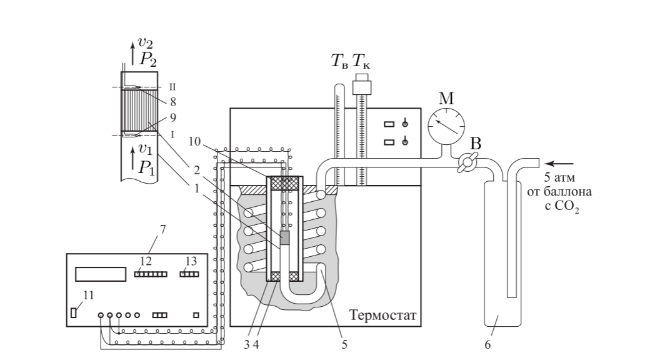
\includegraphics[scale=3]{stand.png}
        \caption{Схема экспериментальной установки для изучения эффекта Джоуля-Томсона}
        \label{stand}
    \end{figure}
    Схема используемой установки приведена на рис. \ref{stand}. Основным
    элементом установки является трубка 1 с пористой перегородкой 2, через
    которую пропускается исследуемый газ. Трубка имеет длину $L = 80$ мм и
    сделана из нержавеющей стали в силу ее малой теплопроводности. Диаметр
    трубки $d = 3$ мм, толщина стенок 0.2 мм. Толщина трубки $l = 5$ мм 
    подобрана так, чтобы обеспечить оптимальный поток газа при перепаде
    давлений $\Delta P \le 4$ атм, при этом в результате эффекта Джоуля-Томсона
    создается достаточная разность температур. 
    \par Давление газа измеряется измеряется манометром М и регулируется 
    вентилем В. Манометр М измеряет разность с атмоферным давлением 
    $\Delta P = P_1 - P_2$.
    \par Разность температур газа до перегородки и после нее измеряется 
    дифференциальной термопарой медь -- константан.

    \section{Ход работы}
\end{document}
